\chapter{Tribal NeuroSim: Foundations and Architecture}

\section{Objectives and Research Connection}

Tribal NeuroSim is the direct continuation of the PremadeGraph graph-analysis pipeline. The PremadeGraph pipeline characterises each player cluster with a set of performance metrics: combat efficiency, resource management, objective control, risk tolerance, and team coordination. These values aggregate into cluster-level metrics (\textit{A\_combat}, \textit{A\_resource}, \textit{A\_map\_objective}, \textit{A\_risk}, \textit{A\_team}), which form the initial genome sequence for tribes in Tribal NeuroSim.

Both dataset clusters appear simultaneously in the simulation. The research question: if cluster profiles derived from Flex Queue and SoloQ compete under identical simulation rules, does the underlying graph structure produce a measurable difference in the emerging survival strategies?

The experimental framework is an exploratory transfer study \cite{bonabeau2002}. It does not attempt to directly predict real match outcomes and does not posit psychological or sociological causality.

\section{Agent-Based and Multi-Agent Model}

Tribal NeuroSim is an agent-based model (ABM): each tribe is an independent decision-making entity that acts solely on the basis of its own local state and immediate spatial neighbourhood. Macro-level patterns (expansion, wars, empire formation, extinction) emerge exclusively as the aggregate of individual decisions \cite{bonabeau2002}.

The system is also interpretable as a multi-agent system (MAS) \cite{wooldridgejennings1995}: each tribe operates as an independent agent with its own internal state, its own local perception, and its own decision logic (neural network). There is no direct communication between agents: interaction occurs exclusively through the shared spatial substrate.

The simulation consistently follows the same structural phases: early expansion (ticks 0--300), consolidation (ticks 300--1000), then imperial wars (tick 1000+).

\section{System Architecture}

\begin{figure}[H]
\centering
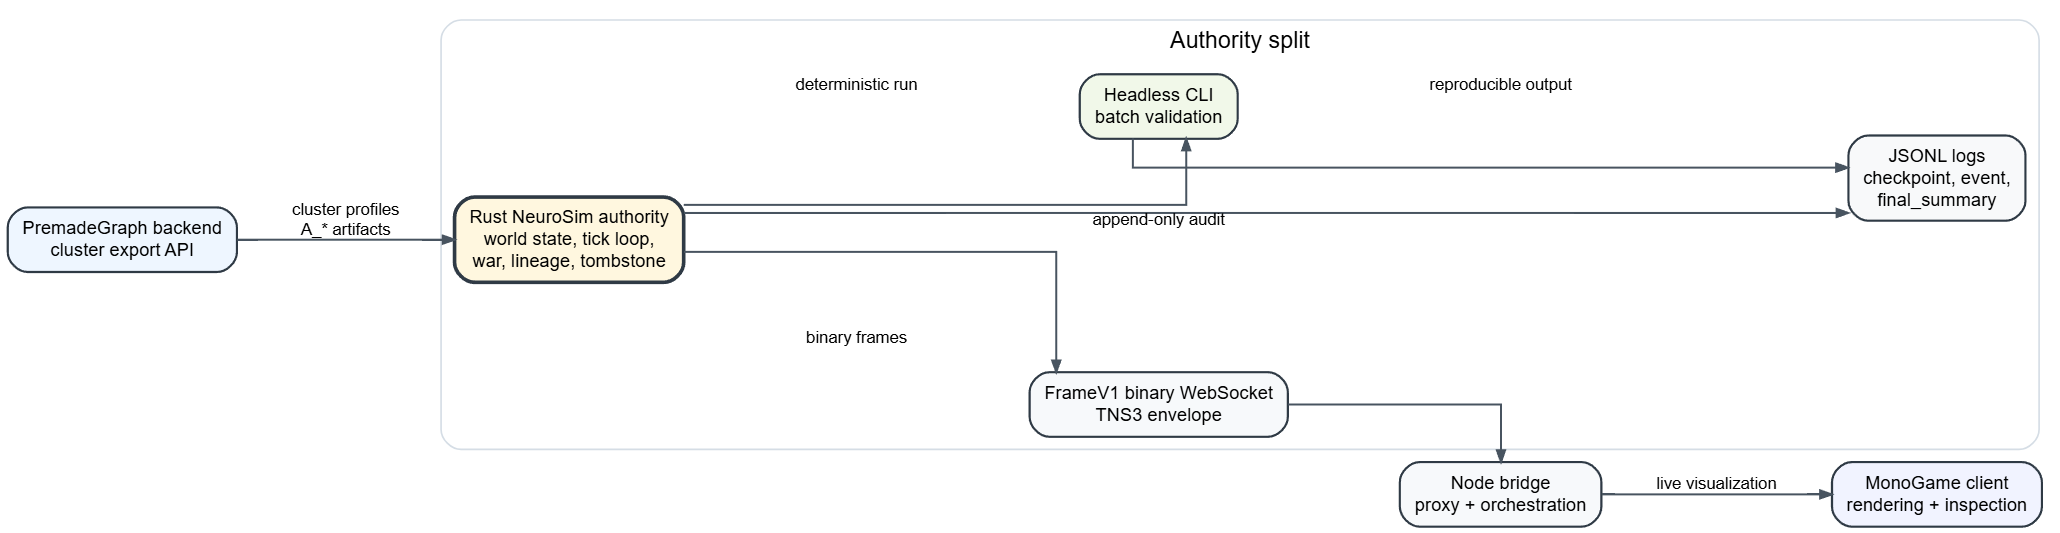
\includegraphics[width=0.92\textwidth]{assets/diagrams/thesis_neurosim_architecture_graphviz.png}
\caption{Tribal NeuroSim responsibility split: the Rust engine is the authoritative source of simulation state, while the Node and MonoGame layers act as intermediary and display.}
\label{fig:neurosim-architecture-graphviz}
\end{figure}

The \textbf{Rust runtime} is the single source of authority: the tick cycle, world state, tribal neural decision-making, war and alliance resolution, fusion logic, tombstone entries, and event logging are all handled by the Rust binary \cite{jung2020}. The \textbf{C\# MonoGame client} is exclusively for visualisation and operator interaction. The \textbf{Node layer} is a thin intermediary: a bridge between MonoGame and the Rust server.

This division is the direct lesson of the browser-based v2 prototype: when simulation state was coupled to the UI layer, ghost wars, memory leaks, and non-deterministic behaviour emerged.

The ghost war specifically meant that two tribes simultaneously observed different war states: one considered the clash finished while the other still treated it as ongoing. The cause was that the UI held the simulation state, and state could drift between HTTP requests. In the current architecture every decision is made in the Rust binary; the MonoGame client only renders the most recently received frame, eliminating drift and making the simulation reproducible from the same initial state at any point.

\section{FrameV1 Binary Protocol}

The Rust server and the MonoGame client communicate via binary WebSocket frames. Each frame begins with a 40-byte \textit{TNS3} envelope (little-endian):

\begin{table}[H]
\centering
\caption{FrameV1 desktop envelope header.}
\label{tab:framev1-envelope}
\begin{tabular}{|r|l|l|}
\hline
\textbf{Offset} & \textbf{Size} & \textbf{Field} \\
\hline
0  & 4 B & Magic: \textit{"TNS3"} \\
4  & 2 B & Version: \textit{1} \\
6  & 2 B & HeaderBytes: \textit{40} \\
8  & 2 B & PayloadKind: \textit{2} (\textit{FrameV1}) \\
10 & 2 B & Flags \\
12 & 4 B & PayloadBytes \\
16 & 8 B & Tick (\textit{u64}) \\
24 & 4 B & Generation (\textit{u32}) \\
28 & 4 B & RecordCount (number of living tribes) \\
32+ & variable & V1 payload \\
\hline
\end{tabular}
\end{table}

The binary format decision is performance-driven: the Rust server handles 599 tribe states in under 40~ms while the MonoGame client decodes and renders asynchronously. Avoiding JSON serialisation saves approximately 150--200~kB of unnecessary text overhead per tick in a 599-tribe world.

Details of event-driven observability and the determinism-bug fix (\textit{clusters.sort\_by(|a, b| a.id.cmp(\&b.id)})) can be found in chapter 13 of the extended version \cite{premadegraph-full}.
